\documentclass[main.tex]{subfiles} % Subfile-Class

% ============================================================================== %
%                            Subfile document                                    %
% ============================================================================== %

\begin{document}

% Template

\subsubsection{Grip Controller}
Wie im Abschnitt~\ref{sec:Gesamtuebersicht_Elektro} erwähnt, steuert der Grip
Controller sämtliche Funktionen im Zusammenhang mit dem Greifen und dem Umgang
mit Hindernissen. Die selbstentwickelte Leiterplatte erfüllt folgende Aufgaben:

\begin{description}
      \item[Digitale Ein- \& Ausgänge] Die Leiterplatte ist mit digitalen Eingangs- und
            Ausgangs-Funktionalitäten ausgestattet. Es existieren mehrere digitale
            Eingänge, die eine flexible Konfigurierung zwischen Spannungspegeln von 3,3 V
            oder 12 V erlauben. Die entprellten Eingänge dienen der Detektion des Anschlags
            des Greifers mittels Endschaltern oder Lichtschranken. Des Weiteren sind zwei
            Anschlüsse für Servos vorhanden. Diese Ausgänge sind mit einer Strombegrenzung
            belegt, welche bei einem maximalen Strom von 1,5 A begrenzt wird. Beim
            Erreichen der Strombegrenzung wird dies dem Mikrocontroller mitgeteilt.
            Zusätzlich sind zwei flexible Ausgänge integriert, die eine Einstellung
            zwischen den Spannungspegeln von 3,3 V oder 12 V erlauben. Einer der beiden
            Ausgänge ist für die Detektion von Hindernissen mittels einer Lichtschranke
            vorgesehen.

      \item[Schnittstelle Kommunikation] Die Kommunikation wird durch den Einsatz von UART
            realisiert. Die differenzielle Kommunikation zwischen dem Grip Controller und
            dem Motion Controller erfolgt direkt über Steuerbefehle. Bei möglichen
            Fehlercodes steht der Grip Controller via Motion Controller mit dem
            RaspberryHAT-PCB in Kontakt.

      \item[Spannungsversorgung] Der Grip Controller transformiert die Versorgungsspannung
            mittels eines 12V-DC/DC-Wandlers auf einen Spannungswert von 5,5 V. Durch den
            Einsatz von zwei LDOs werden gefilterte Spannungspegel von 3,3 V und 5 V
            bereitgestellt.

      \item[Sonstige Besonderheiten] Bei der Konzeption dieser Leiterplatte wurde bewusst
            eine grosszügige Reserve an Anschlüssen eingeplant, um auf unvorhergesehene
            Änderungen dennoch genügen Anschlüsse zu bieten. Darüber hinaus ist die
            Leiterplatte mit LEDs ausgestattet, die im Falle einer Fehlersuche den
            Betriebsstatus der jeweiligen Komponenten-Gruppen anzeigen.
\end{description}

Die Abbildung~\ref{fig:GripController_3D} zeigt die 3D-Ansicht des Grip
Controllers.

\begin{figure}[H]
      \centering
      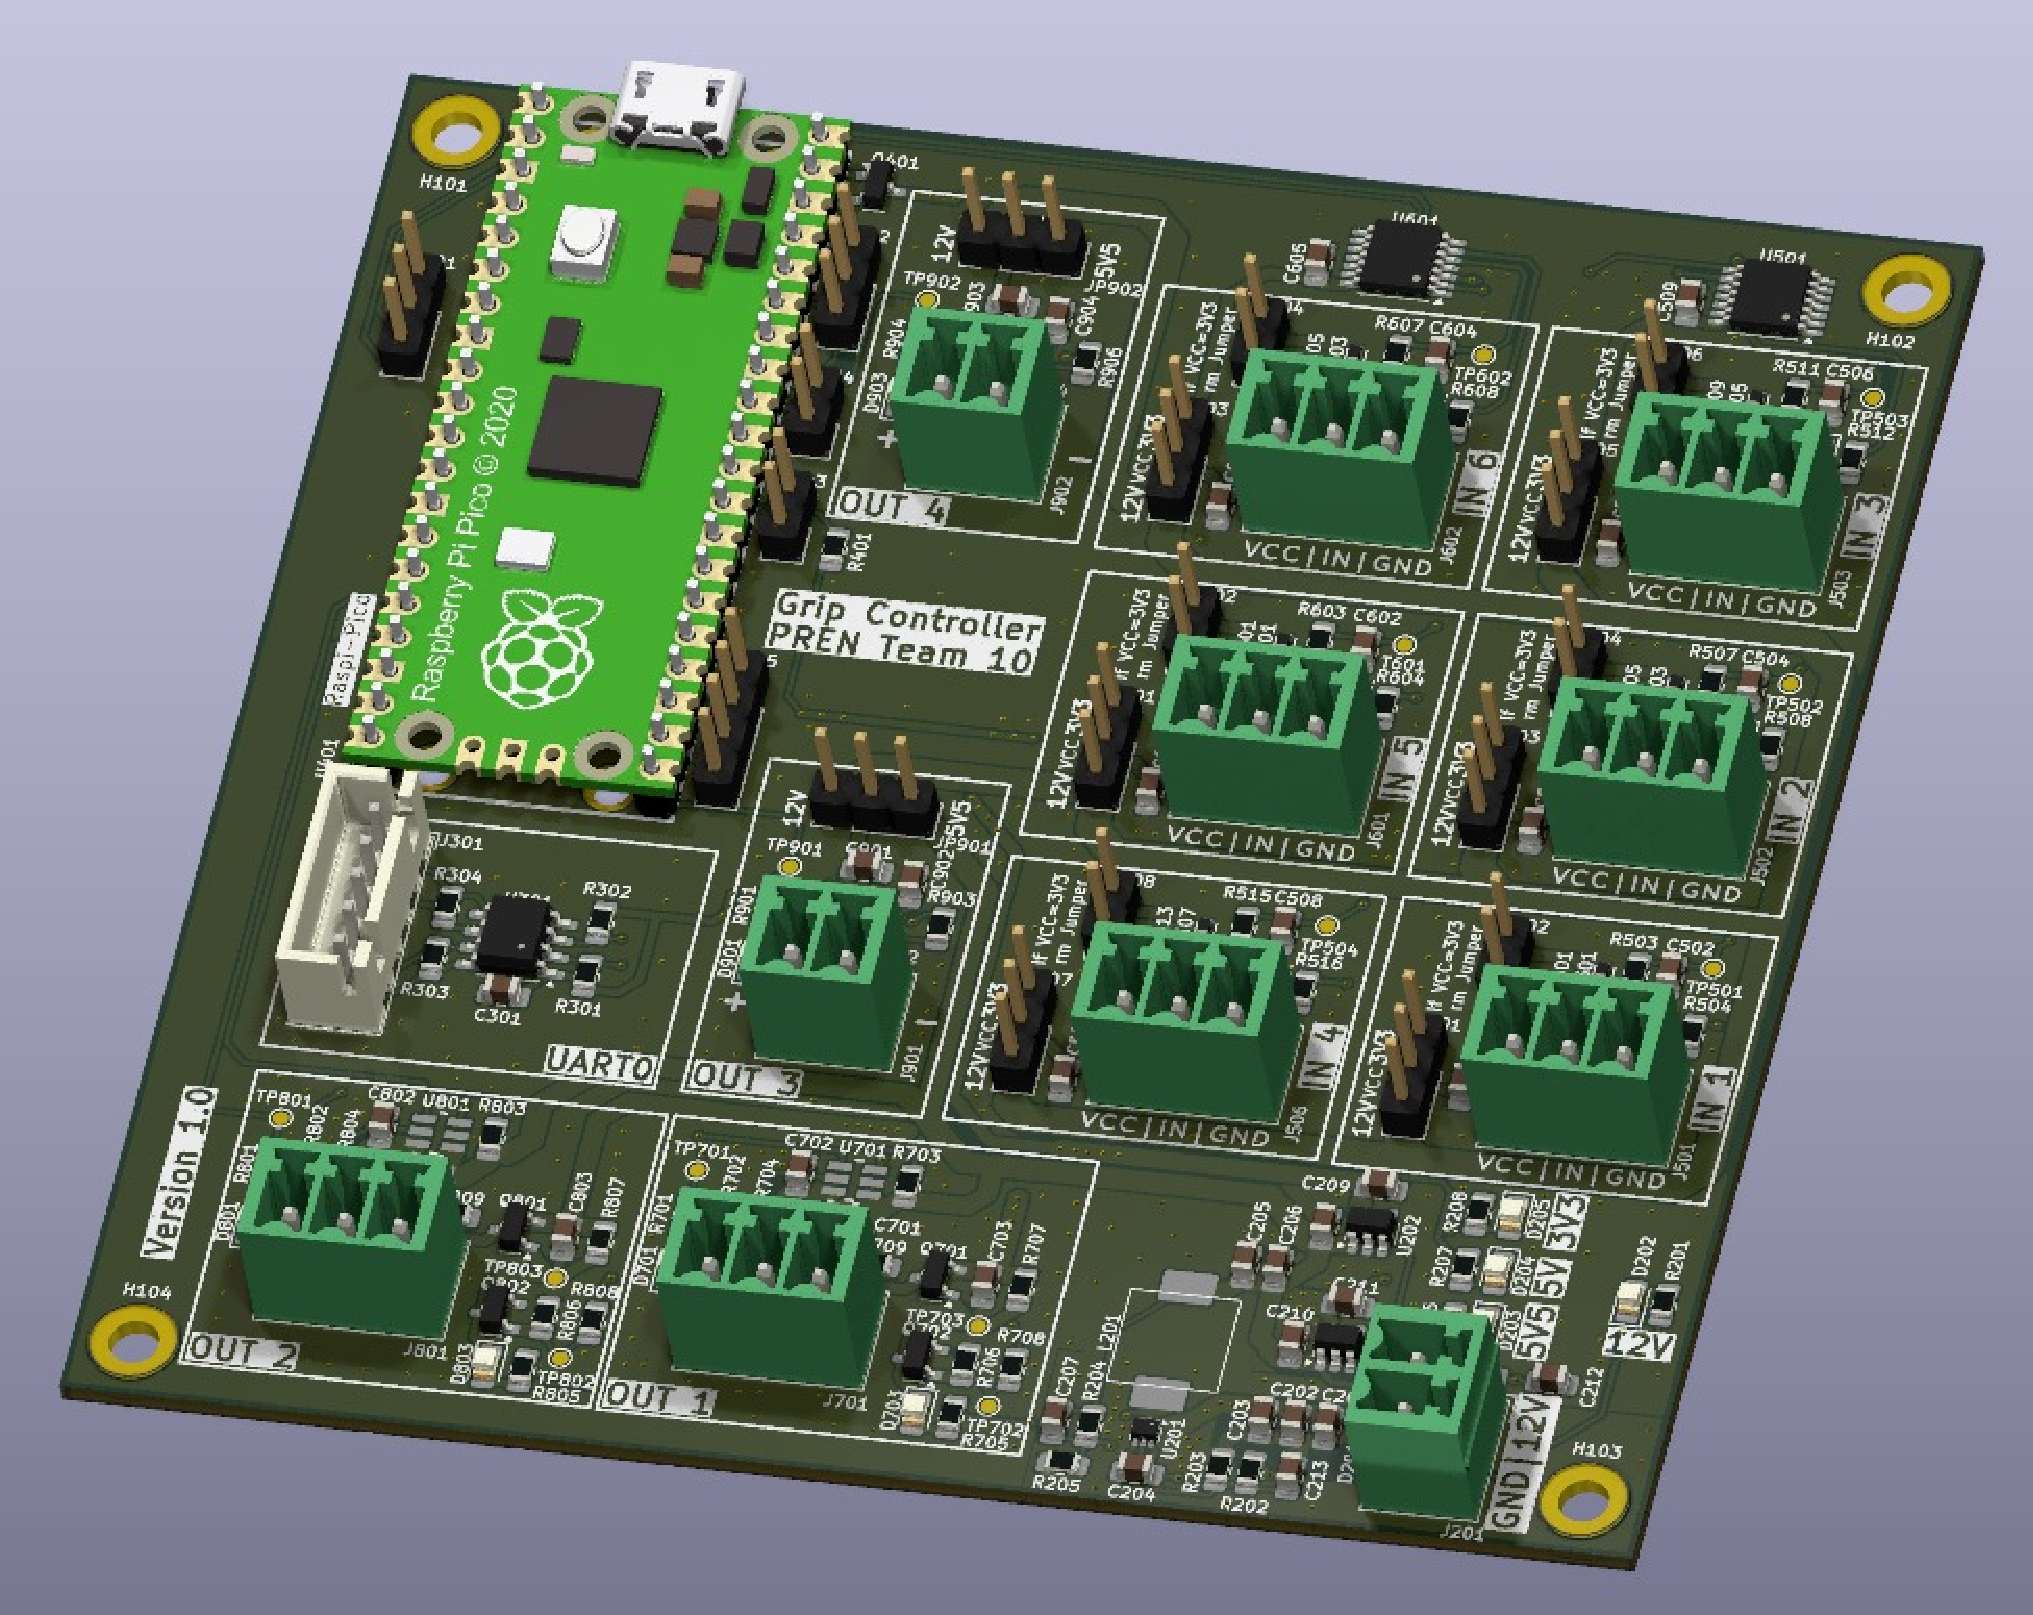
\includegraphics[width=0.75\textwidth]{./fig_GripController/GripController_3D.pdf}
      \caption{3D-Ansicht Grip Controller}~\label{fig:GripController_3D}
\end{figure}

Bei der Entwicklung dieser Leiterplatte wurde auf Teilbaugruppen des Motion
Controllers zurückgegriffen. Alle relevanten Designfiles sind im digitalen
Anhang verfügbar.

\end{document}